In this chapter, we describe the approach which we have adopted to create the dynamic benchmark of executable python software. The overall workflow of the approach is shown in the Figure \ref{fig:overall_approach}.

\begin{figure}[ht]
\centering
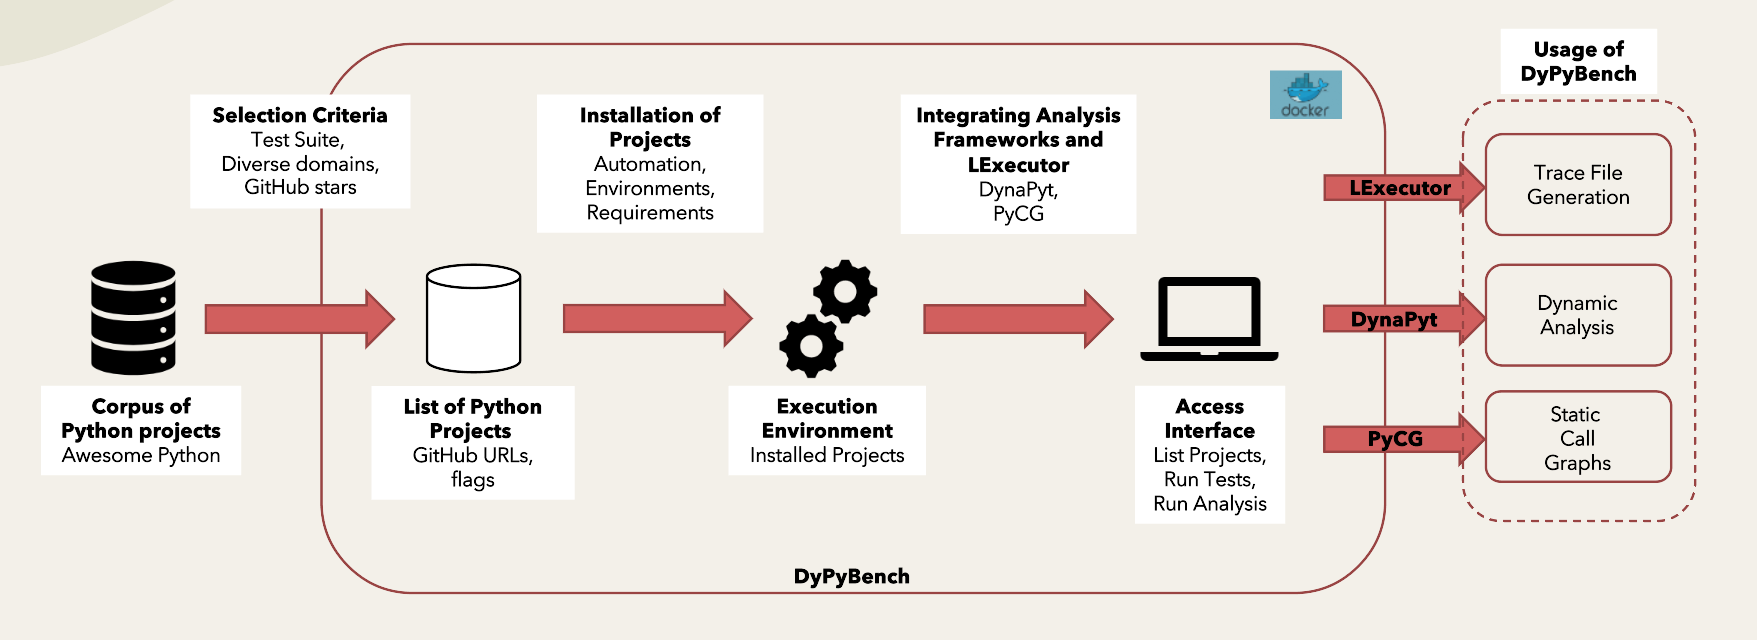
\includegraphics[width=1\linewidth]{figures/approach/DyPyBench3.png}
\caption[Approach]{\label{fig:overall_approach}Overall Approach of DyPyBench}
\end{figure}

As can be seen from the figure \ref{fig:overall_approach}, we first apply the selection criteria to the corpus of python projects to select a number of projects (Section \ref{approach:project selection}.
The list of projects is then used to prepare the benchmark by installing the projects and their dependencies using automation (Section \ref{approach:benchmark preparation}).
We proceed by integrating the two analysis frameworks, DynaPyt and PyCG (Section \ref{approach:analysis framework}). 
We also integrate LExecutor into the benchmark (Section \ref{approach:LExecutor}).
Finally, we package and export the benchmark with an access interface for use by researchers and developers (Section \ref{approach:artifact packaging and interface}).   

With the provided approach, we aim to achieve the properties as listed below.
\begin{itemize}
    \item \textbf{Large-scale} The benchmark should comprise tens of real-world open-source projects, allowing users to evaluate their analyses on a wide range of code.
    \item \textbf{Diverse} The benchmark should contain projects from a diverse range of application domains that reflect the state of today's Python ecosystem.
    \item \textbf{Ready-to-run} There should be a single interface to run each project in the benchmark, making it easy for users to set up and execute the entire benchmark.
    \item \textbf{Ready-to-analyze} To enable dynamic analyses, the executions of all projects in the benchmark should be set up to be analyzed.
    \item \textbf{Compositional} To help users understand the behavior of specific projects or even individual test cases, it should be easy to run subsets of full benchmark.
    \item \textbf{Long-term} The benchmark should be built using commonly used tools and formats, e.g., pip and Docker, to ensure its longevity.
    \item \textbf{Extensibility} The benchmark should be easily extensible, allowing users to add, remove or update the tools, frameworks and projects.  
\end{itemize}

\section{Projects Selection}
\label{approach:project selection}
In this section, first we discuss about the available python projects and why we use awesome-python as a corpus for our benchmark (Section \ref{approach:corpus of python projects}).
Then we discuss about the three selection criteria which we use to select projects from the corpus to make our benchmark diverse and large-scale (Section \ref{approach:selection criteria}).
\subsection{Corpus of Python Projects}
\label{approach:corpus of python projects}
Python's ease of use and popularity, as well as the usage in different domains has led to a large number of projects being developed and made available to the community as open-source projects.
GitHub alone contains a lot of open-source repositories that have python as their primary programming language.
Furthermore, there are some GitHub repositories which provide a collection of python projects such as Awesome Python \footnote{https://github.com/vinta/awesome-python/}, Awesome Python Applications \footnote{https://github.com/mahmoud/awesome-python-applications} and Python Projects \footnote{https://github.com/practical-tutorials/project-based-learning}.
These collections of projects also provide us with a classification for the projects based on the application domains.
In this work, we use the awesome-python project which contains a curated list of some of the awesome open-source python projects including libraries, frameworks and software. 
The awesome-python project is the corpus of projects for our benchmark as it contains a collection of 679 python projects.
Awesome-python further classifies these projects into 92 main categories, out of which some of the categories are further divided into sub-categories.
These sub-categories contain the subset of the main category based on technology, tool and their intended usage.
For example, the sub-categories for Distributed Computing are Batch Processing and Stream Processing which are the two intended ways of processing data.
The top 10 categories and the number of projects in those are listed in table \ref{table:awesome-python}.
Appendix \ref{appendix:awesome python projects} provides more details on the various categories and number of projects in each category provided by awesome-python project.

\begin{table}[ht]
    \centering
    \begin{tabular}{lc}
    \hline
    \textbf{Category} & \textbf{Number of Projects}\\
    \hline
    Testing & 30\\
    Text Processing & 22\\
    Science & 21\\
    Code analysis & 18\\
    Debugging Tools & 18\\
    Specific Formats Processing & 18\\
    Command Line Tools & 17\\
    GUI development & 16\\
    Database Drivers & 15\\
    Image Processing & 15\\
    \hline
    \end{tabular}
    \caption{Top 10 Project Categories (Awesome Python)}
    \label{table:awesome-python}
\end{table}

\subsection{Selection Criteria}
\label{approach:selection criteria}
To select projects for our benchmark, we use three criteria namely diverse domain, test suite execution with pytest and GitHub stars.
To ensure the diversity property presented before, we sample the projects from across multiple categories covering as many application domains as possible provided by the awesome-python corpus.
Since, in this work we are creating a dynamic benchmark we focus on the projects for which we can perform execution.
Test suites provide us with files that can easily execute the code using testing libraries such as pytest and unittest.
Thus we select projects with test suites which can run using the popular pytest library that is also compatible with unittest. 
Lastly, to ensure the criterion of GitHub stars, we select projects which have at least 500 stars on its GitHub repository. 
The number of stars a project has on GitHub is an indication of how popular and well-regarded it is in the community.
More stars generally mean more people have found the project useful and it has a larger user base and community of contributors \cite{github_stars}.
We find 500 stars to be sufficient since it allows us to have the required number of well-regarded projects.  

\section{Benchmark Preparation}
\label{approach:benchmark preparation}
In this section, we start with a discussion about how we use flags in a list of projects to automate the installation process (Section \ref{approach:list of projects}).
We then discuss about how we use these flags in our work to install 50 projects (Section \ref{approach:bash scripts}).
Finally, we discuss about the working environment which is created by the installation of the above 50 projects (Section \ref{approach:collection of projects}).
\subsection{List of Python Projects}
\label{approach:list of projects}
Applying the selection criteria as described before, we select 50 open-source python projects.
Although, the installation and setup of these projects follow similar steps, there are certain differences which vary from project to project.
For example, the path and the name of requirements file to install dependencies varies for each project.
Some of these differences can be attributed to the directory structure of source code present in the GitHub repository.
In order to automate the process of installation and setup of projects, we need a way to work around these differences for each project.
In this work, we use a list with specific flags inside a text file to handle the aforementioned differences.
This structure of a single entry  which represents one project in this list is $ \textbf{project\_url requirement\_flag *requirement\_file test\_suite} $.
In the structure, \textit{project\_url} corresponds to Git URL for the project, whereas \textit{requirement\_flag} represents the information pertaining to the presence or absence of requirement file.
The \textit{requirement\_flag} can have 2 possible values, \textit{rt} and \textit{t}.
The next flag in the entry is the \textit{requirement\_file}, which is the path of requirement file. 
This flag is optional and is present only when the \textit{requirement\_flag} is \textit{rt}.
The final flag in the entry is \textit{test\_suite} that contains the path of the test directory which is needed to execute tests.
Furthermore, it is easy to add, modify or delete an entry from the text file which makes the benchmark extensible.
Table \ref{table:list of projects} shows two example entries in the list.
The first entry is a project with a requirement file present at src/requirements.txt and test suite in the directory tests, while the second entry does not contain a requirement file and its test suite is present in the directory src/tests.

\begin{table}[ht]
    \centering
    \begin{tabular}{llll}
    % \hline
    % \textbf{GitHub URL} & \textbf{Flag} & \textbf{Requirement File} & \textbf{Test Path}\\
    \hline
    https://github.com/test/test-project.git & rt & src/requirement.txt & tests\\
    https://github.com/tester/test-project.git & t & src/tests\\
    \hline
    \end{tabular}
    \caption{List of Projects (Collection Text File Structure)}
    \label{table:list of projects}
\end{table}

\subsection{Installation of Projects}
\label{approach:bash scripts}
The above list of projects with the specified flags in a text file is used to automatically install the projects with a single command.
With the URL to the GitHub Repository and optional requirement file, we perform a series of steps to install each project with its required dependencies.
Firstly, we clone the repository from the URL provided in the text file to get the source code.
We then create a virtual environment to avoid dependency conflicts between different projects.
Then we install the project to the virtual environment using the source code cloned before. 
Finally, if there is a requirement file we install the dependencies specified in this file to the virtual environment.
The mundane and repetitive task of performing these steps for each of the 50 projects is automated using scripts.
Scripts can handle repetition through the use of loops such as for and while.
They can also work with exceptional cases using conditionals such as if else statements.  

\subsection{Execution Environment}
\label{approach:collection of projects}
The automated installation of projects provide us with a collection of 50 python projects.
This collection forms the pool of projects which our benchmark provides to perform code analysis or to generate training data for neural models.
Each project installed using the automation is present inside a sub-folder in the collection.
This makes it easier to work on individual projects when needed.
When a particular project from the collection needs to used, a duplicate copy of the same is created.
This ensures the long-term usage of the projects in the benchmark by preserving the projects and their virtual environments.
The dynamic nature of python and open-source ecosystems results in frequent changes to the projects.
Another advantage provided by duplication is avoiding the re-installation of projects which saves significant time and effort. 

\section{Integrating Analysis Frameworks}
\label{approach:analysis framework}
To satisfy the property of ready-to-analyze, we need to integrate some code analysis frameworks into our benchmark.
In this work, we inncorporate two such frameworks, namely, DynaPyt,  which a general purpose dynamic analysis framework and PyCG, which is a static analysis framework to generate call graphs.
The following sections explain the integration of these two frameworks.
\subsection{DynaPyt}
In this work, we use DynaPyt to perform dynamic analysis for generating call graphs.
We first develop the Call Graph Analysis using the function pre\_call hook provided by DynaPyt.
This is then used to instrument the source code of the project.
Finally, the test suite of the instrumented project is executed which generates a run-time call graph.
The steps of instrumentation and execution of tests is integrated into the access interface. 

\subsection{PyCG}
In this work, we use PyCG to generate call graphs for the collection of projects.
The test files are provided as the entry point for generating the the call graphs.
The required arguments and command to generate the call graphs based on static code analysis is integrated into the access interface.

\section{Integrating LExecutor}
\label{approach:LExecutor}
While code analysis provides a usage scenario of our benchmark, we add another usage scenario of collecting data for fine-tuning a neural model.
This is done using LExecutor, which provides a command to fine-tune the model and improve its accuracy using the training data.
In this work, we first instrument the project which we need to add into the training data.
We then run the test suite of the instrumented project, which generates one or more trace files.
These trace files are then fed to the LExecutor which provides a command to use the trace files and generate training data.
The instrumentation and test suite execution are integrated into the access interface provided by the benchmark.

\section{Artifact Packaging and Interface}
\label{approach:artifact packaging and interface}
In this section, we first provide the details regarding the access interface we design to provide make the benchmark easily accessible (Section \ref{approach:access interface}).
Then we talk about why we use Docker to package and export our benchmark and how it makes the benchmark extensible (Section \ref{approach: packing and exporting}).

\subsection{Access Interface}
\label{approach:access interface}
To provide an easy access to the projects and the analysis frameworks in the benchmark, we create a single command line access interface.
Along with easy access, we also aim to make the benchmark ready-to-run and ready-to-analyze with this interface. 
The access interface provides various alternatives to the end user specified by the command line options.
The available options are provided in the table \ref{table:access interface options}, where the first column specifies the option and the second column provides description of its usage.
With the options \textit{dynapyt\_instrument}, \textit{dynapyt\_run}, \textit{lex\_instrument}, \textit{lex\_test} and \textit{pycg}, one can specify a variable number of projects which makes the benchmark highly versatile.

\begin{table}[ht]
    \centering
    \begin{tabular}{ll}
    \hline
    \textbf{Option} & \textbf{Description}\\
    \hline
    list    & List the project number, name and GitHub URL\\
    test    & Run test suite of specified projects\\
    save    & Save standard output and error to file specified\\
    timeout & Timeout in seconds for commands\\
    update\_dynapyt\_source   & Clone or update source code of DynaPyt\\
    update\_lex\_source   & Clone or update source code of LExecutor\\
    dynapyt\_instrument  & Instrument files for DynaPyt\\
    dynapyt\_file    & Specify file to use for instrumentation of DynaPyt\\
    dynapyt\_analysis    & Specify the analysis to perform for DynaPyt\\
    dynapyt\_run & Execute DynaPyt analysis for specified projects\\
    lex\_instrument  & Instrument files for LExecutor\\
    lex\_file    & Specify file to use for instrumentation of LExecutor\\
    lex\_test    & Execute LExecutor for specified projects\\
    pycg    & Execute PyCG for specified projects\\
    \hline
    \end{tabular}
    \caption{Access Interface (Command Line Options)}
    \label{table:access interface options}
\end{table}

\subsection{Packaging and Export}
\label{approach:packing and exporting}
In order to use the benchmark readily, it should contain all of its constituent parts and must be easy to setup.
In this work, we package the benchmark containing the collection of projects, the analysis frameworks, LExecutor and the access interface into a Docker \cite{Docker_2022} image.
This Docker image can be used to create containers to access the benchmark.  
Since, Docker provides a loosely isolated environment for its containers we install all the operating system related dependencies into the image itself.
The Docker image is then exported on the Docker Hub \cite{docker_hub} repository.
This approach of using Docker image also makes the benchmark long lasting, since the image is available long after the release.
Another advantage of using Docker is the simplicity of modifying the benchmark as per the need of the user.
For example, one can add another analysis tool or change some projects in the benchmark or add new test cases for some projects.
All of these can be done by importing the Docker image and making the changes as per the needs of the developer or a user.
This makes our benchmark easily extensible.